% ---------------------------------------------------------------------------
%                   LATEX TEMPLATE FOR MARL PhD THESIS
% ---------------------------------------------------------------------------

% Taemin Cho put together a nice LaTeX class, that Oriol Nieto modified.
% Eric Humphrey added all of this sweet content, and made it available to 
% the rest of MARLities.

% Everything is based on Harish Bhanderi's PhD/MPhil template, then Uni Cambridge
% http://www-h.eng.cam.ac.uk/help/tpl/textprocessing/ThesisStyle/
% corrected and extended in 2007 by Jakob Suckale, then MPI-CBG PhD programme
% and made available through OpenWetWare.org - the free biology wiki

%: Style file for Latex NYU-MARL:
% This template package can be found in ./Latex/Classes/
% It aims to follow the official NYU-Steinhardt guidelines:
%       http://steinhardt.nyu.edu/doctoral/dissertation/formatting
\documentclass[oneside, 12pt, letterpaper]{marl}
% preamble
\usepackage[default,regular,black]{sourceserifpro}



\proposaltitle{\doublespacing 
	Modern Generative Methods for Music Transcription
}

\threecommittee
{Professor Juan Pablo Bello, Chairperson}
{Professor }
{Professor }

\degree{Doctor of Philosophy}
\degreedate{\the\year}

% ----------------------------------------------------------------------
% The section below defines www links/email for author and institutions
% They will appear on the title page of the PDF and can be clicked

%: ----------------------- HELP: www links
% You can also see below how, www links are placed
% \href{http://www.something.net}{link text}

\author{\href{mailto:jongwook@nyu.edu}{Jong Wook Kim}}
\program{Program in \href{http://steinhardt.nyu.edu/music/technology/}{Music Technology}}
\department{Department of \href{http://steinhardt.nyu.edu/music/}{Music and Performing Arts Professions}}
\university{\href{http://www.nyu.edu/}{New York University}}
\crest{}%\includegraphics[width=3in]{NYUlogoLarge2597}}
\submittedtext{Submitted in partial fulfillment\\
  of the requirements for the degree of\\
  Doctor of Philosophy in the\\
  \href{http://steinhardt.nyu.edu/}{Steinhardt School of Culture, Education, and Human Development}}


% ----------------------------------------------------------------------

% turn of those nasty overfull and underfull hboxes
\hbadness=10000
\hfuzz=50pt
\makeindex


%if output to PDF then put the following in PDF header
\ifpdf
\pdfinfo { /Title  (\@title)
	/Author (Jong Wook Kim <jongwook@nyu.edu>)
	/Subject (Music Technology)
	/Keywords (Marzipan, jujubes, pudding, sesame snaps) }
	\pdfcatalog { /PageMode (/UseOutlines)	/OpenAction (fitbh)  }
\fi

\begin{document}

\widowpenalty=10000
\clubpenalty=10000


%: ----------------------- generate cover page ------------------------
%\setstretch{1.2}
\maketitle  % command to print the title page with above variables
% \makecopyright

%: ----------------------- abstract ------------------------

% Your institution may have specific regulations if you need an abstract and where it is to be placed in the document. The default here is just after title.

% 
% Thesis Abstract -----------------------------------------------------


%\begin{abstractslong}    %uncommenting this line, gives a different abstract heading
\begin{abstracts}        %this creates the heading for the abstract page

Put your abstract or summary here, if your university requires it.

\end{abstracts}
%\end{abstractlongs}


% ---------------------------------------------------------------------- 


%: ----------------------- tie in front matter ------------------------
\doublespacing

% % Thesis Dedictation ---------------------------------------------------

\begin{dedication} %this creates the heading for the dedication page

To the Flying Spaghetti Monster.

\end{dedication}

% ----------------------------------------------------------------------

% 
% this file is called up by thesis.tex
% content in this file will be fed into the main document

\chapter*{Acknowledgements}

Sweet sweet sweet roll croissant candy souffle pie chocolate bar.
Pudding candy carrot cake sweet halvah. 
Ice cream ice cream tiramisu jelly-o chupa chups chupa chups carrot cake. 
Donut tootsie roll pie pudding icing muffin candy canes. 
Cupcake tootsie roll croissant chocolate applicake croissant macaroon gummi bears. 
Muffin icing icing toffee jelly beans toffee lemon drops. 
Cookie chocolate cake topping carrot cake chocolate bar jujubes sweet roll.


%: ----------------------- contents ------------------------
% levels are: 0 - chapter, 1 - section, 2 - subsection, 3 - subsubsection
\setcounter{secnumdepth}{3} % organisational level that receives a numbers (NYU Steinhardt recommends level 0, which is pretty hideous)
\setcounter{tocdepth}{2}    % print table of contents for level 2
\singlespacing
\tableofcontents            % print the table of contents
%\addcontentsline{toc}{section}{continued}
%: ----------------------- list of figures/tables ------------------------
\clearpage
\listoftables                   % print list of tables
\clearpage
\listoffigures                  % print list of figures

%: ----------------------- glossary ------------------------

% Tie in external source file for definitions: /frontmatter/glossary.tex
% Glossar entries can also be defined in the main text. See glossary.tex

%% this file is called up by thesis.tex
% content in this file will be fed into the main document

\newacronym{tcap}{TCAP}{Toffee chocolate apple pie}


\newglossaryentry{Chupa chups}
{
  name={chupa chups},
  description= {Powder fruitcake ice cream ice cream brownie biscuit ice cream ice cream}
}

%\makeglossaries
%\clearpage
%\printglossaries

\chapterbegin

%: ----------------------- epigraph ------------------------
% 
\chapter*{}

\begin{quote}
``Marshmallow wafer oat cake carrot cake sugar plum gummi bears jujubes marzipan.''

\end{quote}

\vspace{1in}
\hspace{2in}
-Willy Wonka, {\it Midnight in the Garden of Good and Evil.}

%: --------------------------------------------------------------
%:                  MAIN DOCUMENT SECTION
% --------------------------------------------------------------

% the main text starts here with the introduction, 1st chapter,...

\mainmatter
\doublespacing
%: ----------------------- subdocuments ------------------------

% Parts of the thesis are included below. Rename the files as required.
% But take care that the paths match. You can also change the order of appearance by moving the include commands.

%!TEX root = ../dissertation.tex
% this file is called up by thesis.tex
% content in this file will be fed into the main document

%: ----------------------- introduction file header -----------------------
% the code below specifies where the figures are stored
\graphicspath{{1-introduction/figures/}}

\chapter{Introduction}
\label{ch:introduction}

As listening is a core constituent of human perception, an essential component of artificial intelligence is \emph{machine listening}.
The purpose of machine listening research is to enable computers to process and understand sounds as humans do.
In recent years, there have been an unprecedented amount of successes in the field of \emph{machine learning}, a near-synonym to artificial intelligence with a connotation of statistical and/or probabilistic methodologies, which redefined what a computer vision or natural language processing systems can do and made previously unimaginable applications such as autonomous driving and a superhuman StarCraft-playing AI into reality.

In this context, this thesis focuses on improving the machine understanding of music in order to automatically transcribe music, which largely remains an unsolved problem despite decades of research.
The recent rapid development in \emph{deep learning} research, however, hints at many new possibilities for improving the performance or even achieving human-level accuracy in music transcription.

\section{Statement of Problem}\label{sec:statement}

\begin{figure}
	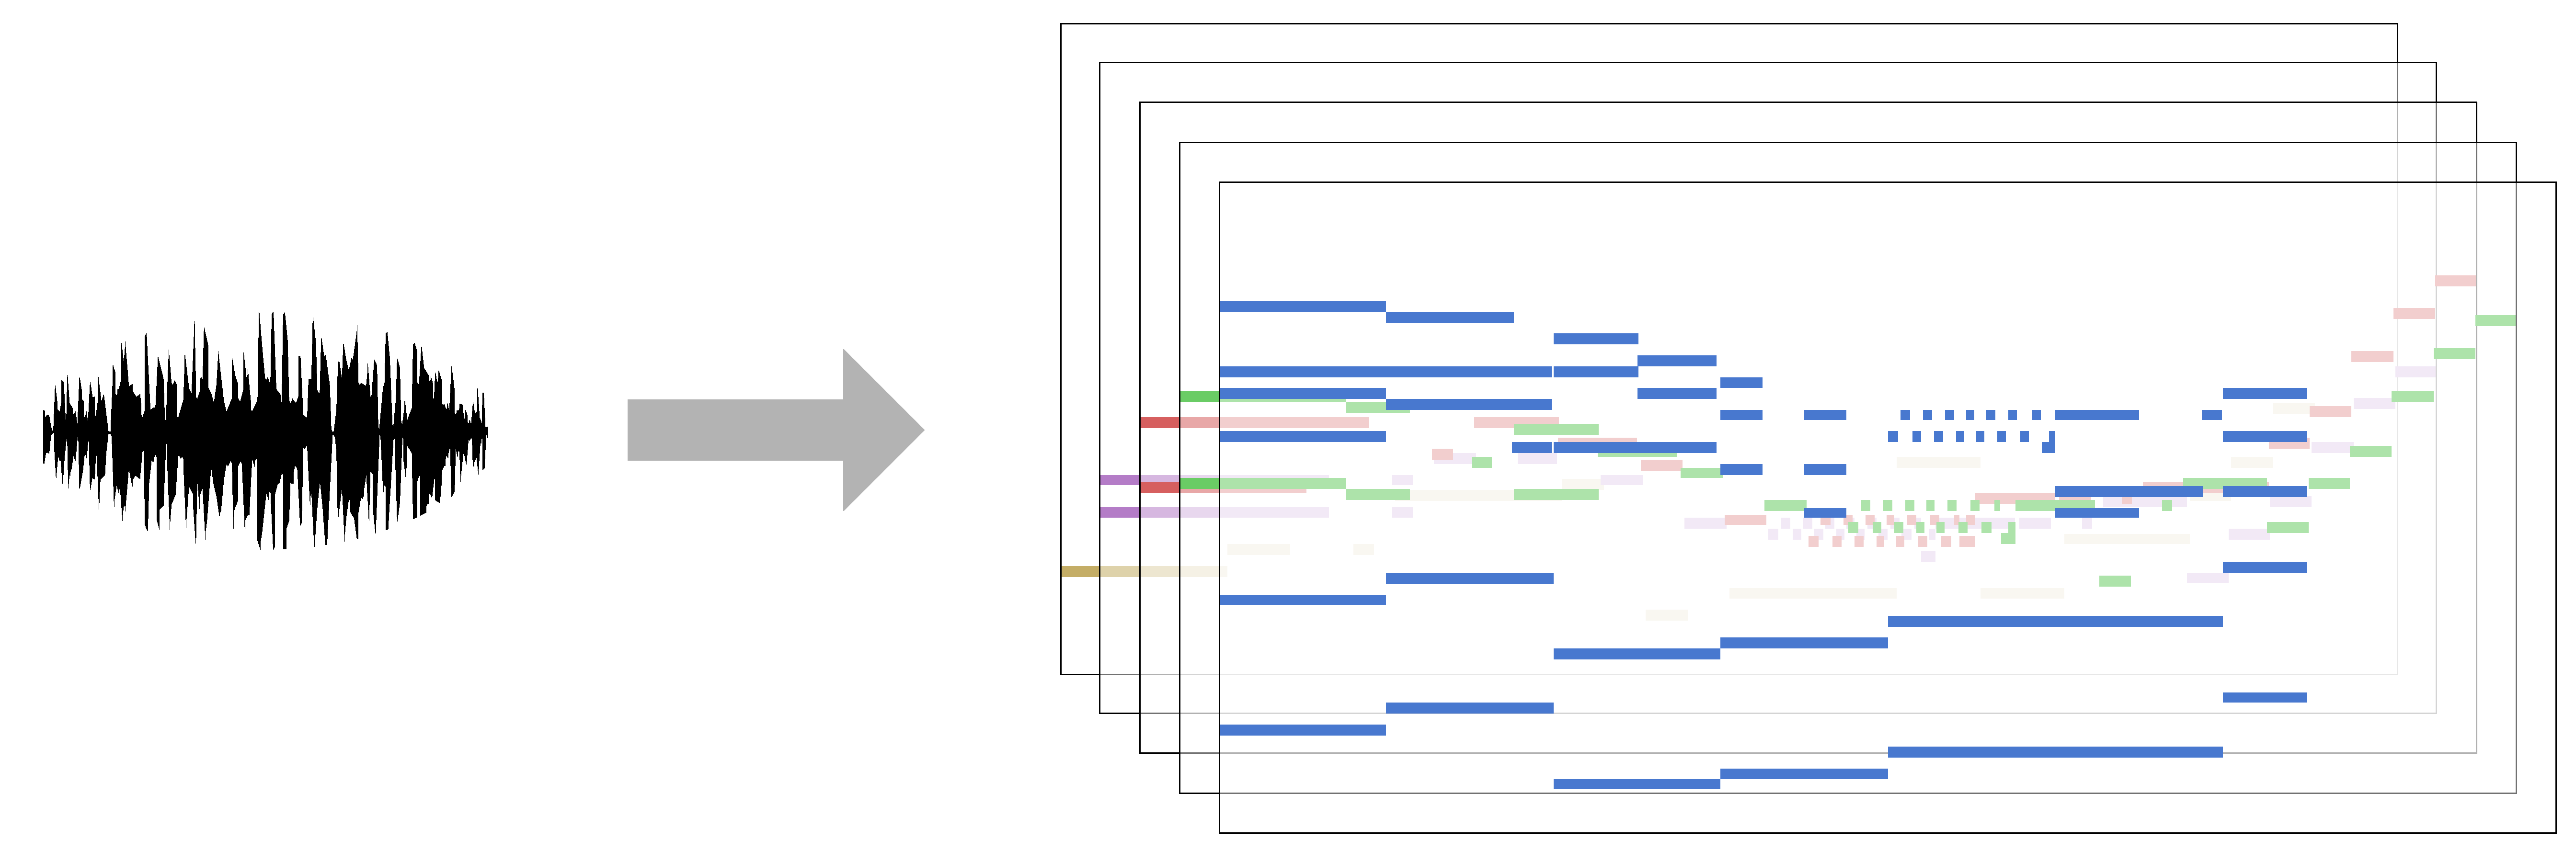
\includegraphics[width=\textwidth]{march-transcription.pdf}
	\caption{The automatic music transcription setup to be used in this thesis. Using per-instrument piano-roll representations is easier for machines to process, and avoids variability and subjectivity that may arise from symbolic and textual notations.} 
	\label{fig:transcription-to-piano-rolls}
\end{figure}

\emph{Automatic music transcription} (AMT) refers to an automated process that can identify musical events in the input audio and convert them into musical notations.
Historically, the definition of automatic music transcription varied by author, usually in terms of the form of the output representation.
In earlier works \cite{moorer1977transcription,piszczalski1977transcription}, the final output of the transcription system was to be the common music notation, i.e. a score, while later literature generalizes the problem by defining it as ``the analysis of an acoustic musical signal so as to write down the pitch, onset time, duration, and source of each sound that occurs in it" \cite{klapuri2006transcription} or ``the process of converting an acoustic musical signal into some form of musical notation" \cite{benetos2013amt}.
This thesis adopts per-instrument piano-rolls as the resulting representation of automatic music transcription, as shown in Figure \ref{fig:transcription-to-piano-rolls}, and defers the ``piano-roll to score" conversion as an out-of-scope task, which involves higher-level nontrivial tasks such as tempo and meter tracking, key signature detection, and music structure identification.
This can be justified since it allows the transcription model to focus on source separation and multi-pitch tracking, which are already highly challenging problems \cite{cemgil2006generative}.


To perform automatic music transcription, various properties of musical events, such as pitch, timbre, harmony, beats, etc., need to be defined and extracted from the audio.
In this sense, the setup of AMT is \emph{discriminative} in nature, meaning that it aims to identify different attributes from given audio, as opposed to \emph{generative} models concerning how to construct audio signals according to given conditions about those attributes.
Meanwhile, when a generative model is jointly trained with an encoder, it can learn to generate data samples from a small number of latent factors, while the encoder learns to extract those factors from the audio in a compact representation, as depicted in Figure \ref{fig:autoencoder}.
Recently, with the increased capacity of machine learning models and hardware, many \emph{deep generative models} have been proposed and shown to be capable of processing high-dimensional multimedia data.
Furthermore, significant research efforts have been made towards learning disentangled representation of data, meaning that the latent factors contain meaningful information that can be easily separated and isolated.
To this end, the goal of this thesis is to study representation learning methods powered by deep generative models, to obtain disentangled information from audio signals that can achieve better performance in music transcription.

\begin{figure}[t]
	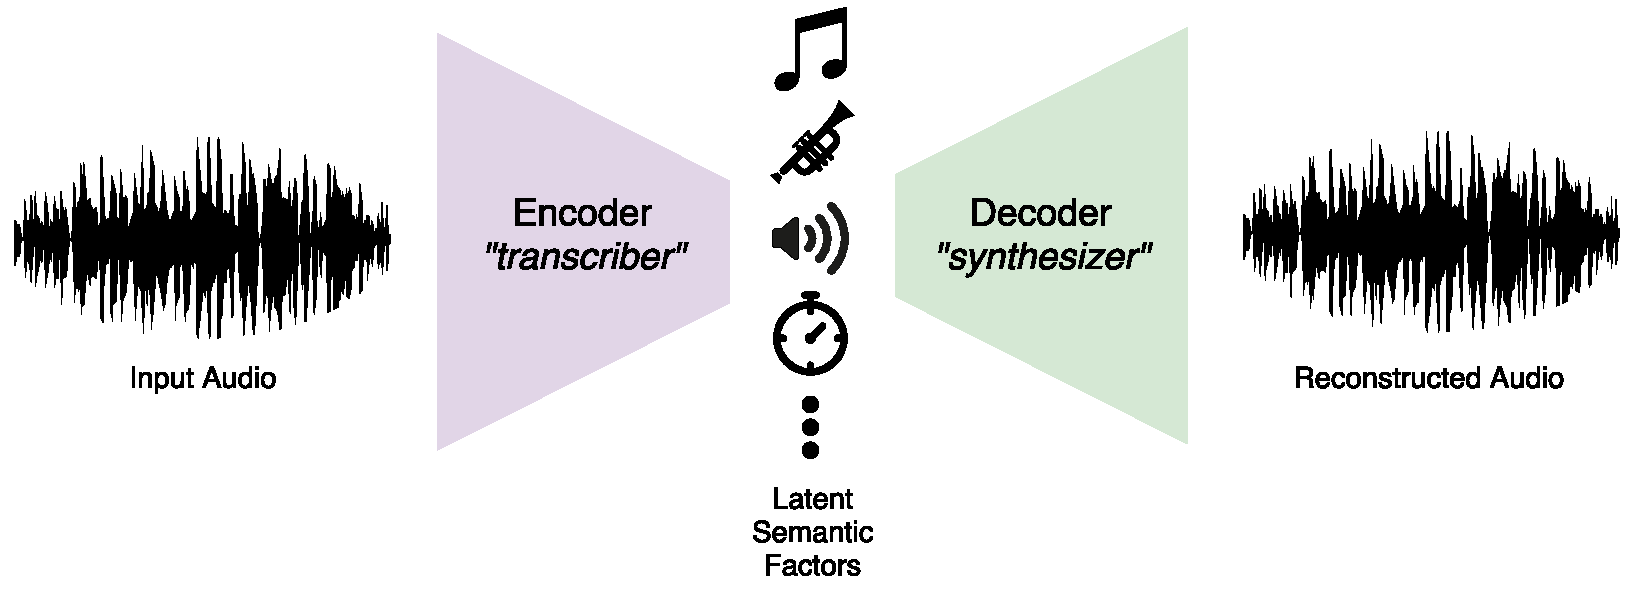
\includegraphics[width=\textwidth]{autoencoder.pdf}
	\caption{A generative model has to know all of necessary information required to reconstruct the audio data, including pitch, timbre, loudness, and duration. Generative models can be jointly trained with an encoder that finds those semantic information, giving a transcriber-synthesizer pair.}
	\label{fig:autoencoder}
\end{figure}

\section{Research Questions}\label{sec:subproblems}

To achieve the goal of improving music transcription with generative models, several research questions needs to be addressed. This thesis considers the following questions regarding the proposed approach towards automatic music transcription.

\vspace{1em}

\begin{enumerate}
\item What kinds of deep models and representations can be used for effectively extracting pitch from audio?
\item How does the choice of datasets affect the accuracy and the generalizability of a trained model?
\item How can we encode the concept of timbre in a way that is useful for music synthesis and transcription?
\item How can a transcription model make informed predictions incorporating the knowledge of music theory?
\item Can a music synthesizer component based on a deep generative model be used to improve music transcription?
\end{enumerate}

\vspace{1em}

We aim to address each of these questions in the technical chapters of the thesis.
Through extensive experimental analysis in each chapter, we draw the conclusion on the effectiveness of deep generative models in the context of automatic music transcription.


\section{Limitations}\label{sec:limitations}

Because of the sophisticated and open-ended nature of automatic music transcription, it is necessary to define the scope of the tasks and data that this thesis will be concerned with.
The purpose of this section is to define those limitations in terms of the scope of music that the proposed AMT system can process, the required capability of symbolic music processing, and the need for perceptual studies regarding the validity of AMT systems.


\subsection{Scope of Music}

Music signals typically contain both harmonic and percussive sources. 
From a signal processing point of view, harmonic sounds are quasi-periodic and contain energy only at certain frequencies, roughly at the multiples of the fundamental frequency, whereas percussive or highly inharmonic sounds have aperiodic frequency spectra in which it is not possible to define a fundamental frequency.
Consequently, transcription models for harmonic sounds and percussive sounds require different techniques according to their nature.


This thesis will limit the focus on the transcription of harmonic sounds and therefore use the per-instrument piano roll notation (Figure \ref{fig:transcription-to-piano-rolls}) as the output representation.
This is a realistic trade-off to make, because of a number of reasons.
First, learning to simultaneously model harmonic and percussive sounds is a harder problem both conceptually and computationally.
Secondly, it is possible to plug a harmonic-only model into a pipeline consisting of HPSS (harmonic-percussive source separation) and a percussion transcription model as an alternative to a comprehensive approach.
Lastly, polyphonic transcription is considered to be the most difficult problem in the domain of automatic transcription, and it is sensible to tackle this as a standalone problem in the simplest possible setup.
Excluding percussive sounds will disallow using most of pop music tracks as-is, but multi-track datasets can still be utilized since they contain each track separately.


Additional limitations should be considered on the types of the instruments and their sound variations.
Depending on the instrument, the same score could be performed using a variety of expressive techniques, such as vibrato, tremolo, pizzicato, and the usage of mutes or harmonics, among others.
In order to accurately produce a piano roll transcription that is invariant to such techniques, the model has to be trained to classify them as nonessential information, requiring the availability of datasets with the annotations for those techniques.
While an ideal model should learn those concepts as humans do, too much timbral or temporal variation for an instrument will prevent the model from learning a consistent representation corresponding to the instrument.
Therefore, for the immediate purpose of this thesis, distributions of music signals that do not contain too much of said variations will be employed.


\subsection{Symbolic Processing of Notes}

As mentioned and justified in the problem statement (Section \ref{sec:statement}), by choosing per-instrument piano rolls as the output of transcription, concerns of symbolic music processing such as beat quantization and score typesetting are excluded from the scope of this study.
The difference between a piano roll output and a full human-readable score output becomes apparent when we compare the piano rolls in Figure \ref{fig:transcription-to-piano-rolls} with Figure \ref{fig:wedding-march-score}, which is the original score from which the piano rolls are plotted.
There are many aspects in producing the score output that are highly subjective and difficult to derive a consistent evaluation metric from, such as the interpretation of legatos or staccatos and the aesthetic choices for typesetting, providing an additional justification for using the piano roll notation.


\begin{figure}
	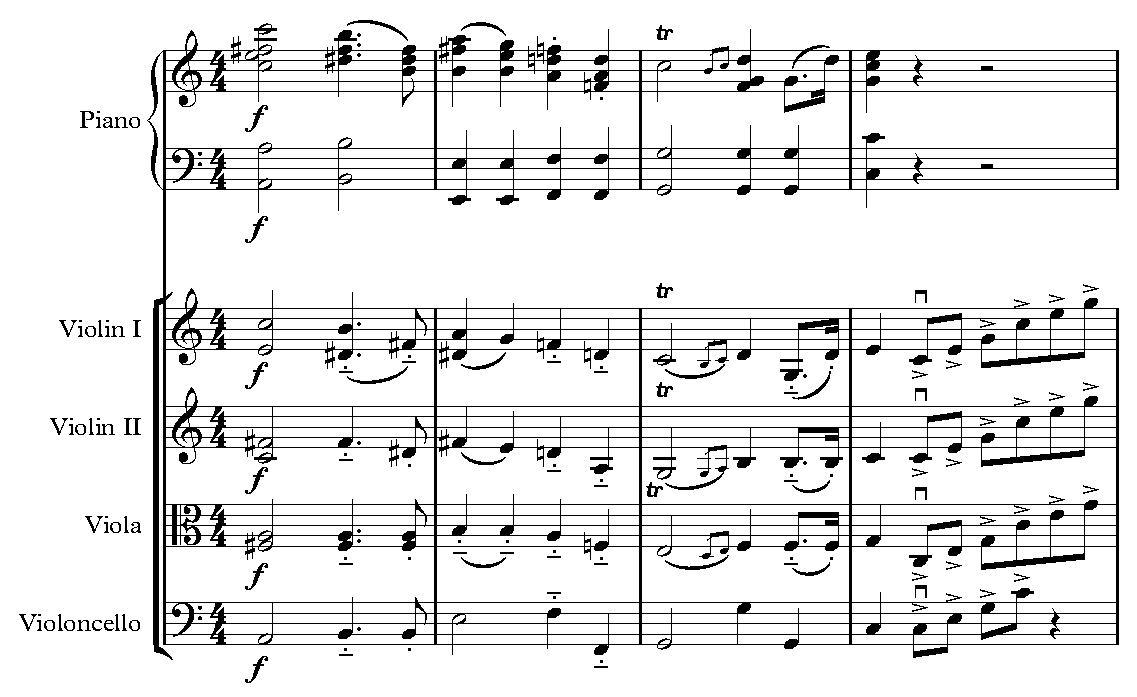
\includegraphics[width=\textwidth]{march-score.pdf}
	\caption{The full score notation of the music used to build the piano rolls in Figure \ref{fig:transcription-to-piano-rolls}. To fully recover this level of notations from the audio, the transcriber has to make many additional decisions than for the piano rolls, such as determining the key signature, time signature, clefs, dynamics, trills, bowing instructions, etc.}\label{fig:wedding-march-score}
\end{figure}


The MIDI file format is suitable for encoding data equivalent to per-instrument piano rolls, consisting of multiple tracks of \texttt{note\_on} and \texttt{note\_off} events with the corresponding timestamps.
MIDI will therefore be a supported output format of the proposed AMT system in addition to the piano roll representations, which can also be conveniently played back by media player software.
Music typesetting software such as Sibelius or Finale can render a MIDI file into score notation using the metadata in the file as well as some heuristics for beat quantization.
However, the readability of the score rendered from a transcribed MIDI file is limited, due to imperfect transcription and the absence of metadata such as the time and key signature.



\subsection{On the Need for Perceptual Studies}

This study of automatic music transcription is entirely quantitative and does not involve subjective tests on human participants.
We only aim to discover the systematic relations between audio signals and corresponding note sequences present in the datasets we use for training.
However, music is essentially a perceived notion, and thus are the core qualities of sound --- pitch, timbre, and loudness --- which are the output of automatic transcription.
For this reason, manually annotating polyphonic music is an error-prone process, where any two annotators may produce drastically different annotations.
Although this problem of inaccuracy and subjective difference is often overcome by using a ground-truth dataset synthesized from known frequency information, the gap still persists between what a model can learn from synthesized audio and how it will respond to real-world sounds.
This thesis uses both kinds of datasets, from synthesized and recorded audio signals, and thus the real-world applicability of each of the proposed models should be carefully examined.

The goal of automatic transcription is at a lower level than for tasks such as  chord recognition and melody tracking, which may incur even more subjective disagreements caused by the imprecise definitions of chords and melodies.
Being directly related to the physical concept of fundamental frequency, pitch is relatively precisely defined in this sense, and formulating automatic music transcription as an audio-to-piano-roll conversion mostly eliminates the ambiguity that exists in chord recognition and melody tracking.
There exist some cases where the mathematical definition of fundamental frequency still cannot be applied for all pitched sounds, such as the Shepard tone \cite{shepard1964circularity} where the pitch of a harmonic sound fails to be consistently mapped to a fundamental frequency.
However, disregarding these few edge cases, this study assumes that the piano roll notation can convey an objective transcription for many practical purposes, allowing us to postulate AMT as a mathematical problem which does not require experiments on human subjects.

\section{Need for Study}

The nature of music transcription is multifold; to create a complete transcription, one has to identify all instruments, onsets, dynamics, and the pitch traces for every instrument present in the music, and it would still be far from achieving the human-level accuracy.
The need for this study arises naturally, not only because this is an intriguing problem in the intersection of music and technology that has remained unsolved for decades, but also because the solution to this problem can provide practical benefits to many applications.

In order to bolster the need for this study, a few of such applications are introduced in this section, followed by discussions on the advantages of employing generative models as a means of better capturing musical semantics.
A brief perspective on AMT is presented in the context of wider AI research, followed by the organization of the chapters.


\subsection{Applications of Automatic Music Transcription}\label{sec:applications}

Many applications of the techniques in the realm of automatic music transcription is on interactive music systems.
\citeA{vercoe1984performer} proposed a quest for a \emph{synthetic performer}, which can listen, perform, and learn in the context of live performance.
Relevant sub-fields include automatic \emph{real-time accompaniment} \cite{dannenberg1985accompaniment} based on dynamic programming was one of the first successful demonstrations of AMT techniques, and \emph{Score following}, a general term referring to the synchronization of a computer with a performer playing a known score \cite{orio2003following}.
An offline music-to-score matching algorithm can also be applied to intelligent audio editors \cite{dannenberg2003following}.

\emph{Music recommender systems} can combine many kinds of information for improved music retrieval and personalization \cite{celma2010music}.
Content-based music recommender systems can utilize not only the metadata but also the audio content, and methods using timbral \cite{magno2008recommendation}, temporal \cite{li2007recommender}, and tonal features \cite{lu2009recommendation} have been introduced.
These music recommender systems can be further improved when the complete information on each domain is made available through AMT.

AMT system can help create databases for query-by-humming \cite{ghias1995humming} by automatically estimating melody annotations, where users can retrieve music by humming an excerpt of the song.
Such databases can also facilitate large-scale musicological analyses \cite{abdallah2015british}, as well as the development of computer-aided music composition \cite{agostini2013aid} that incorporates musicological knowledge.


\subsection{Generative Modeling for Fully Capturing Semantics}

Being ``generative'' means that a model is capable of generating new samples in the domain of the original data.
Generation in the symbolic domain creates new musical scores, and a generative model in the audio domain creates audio waveforms.
These two kinds of generative systems are familiar to computer music artists and are referred to as algorithmic composition \cite{fernandez2013ai} and sound synthesis \cite{cook2002synthesis} models.
This thesis defines the term ``generative model'' more specifically, as a model that can learn the distribution of provided data and can sample new samples in the original distribution.
This differs from the term ``generative'' used in computer music in a sense that it aims to accurately model the probability distribution and learn to regenerate the real-world audio to be used in music transcription, rather than focusing on the artistic aspects of generating new kinds of sounds and music.

By learning to generate data using fewer parameters than the scale of the dataset, a model has to discover the underlying natural features from the distribution of data.
In music transcription, these features correspond to the musical concepts such as pitch, timbre, and rhythm.
Philosophically, this idea follows what Richard Feynman once wrote on his blackboard, \emph{``What I cannot create, I do not understand''} and \emph{``Know how to solve every problem that has been solved''}.
He meant that the marker for truly understanding something is the ability to construct it completely from scratch.
Generative models are a branch of unsupervised learning, because they do not require labeled data.
\citeA{lecun2016unsupervised} introduced unsupervised learning as a cake, with supervised learning as icing and reinforcement learning as the cherry on the top, by which he meant that generative models need to predict at a much larger scale of information and should be is able to learn the ``common sense''.

\begin{figure}
	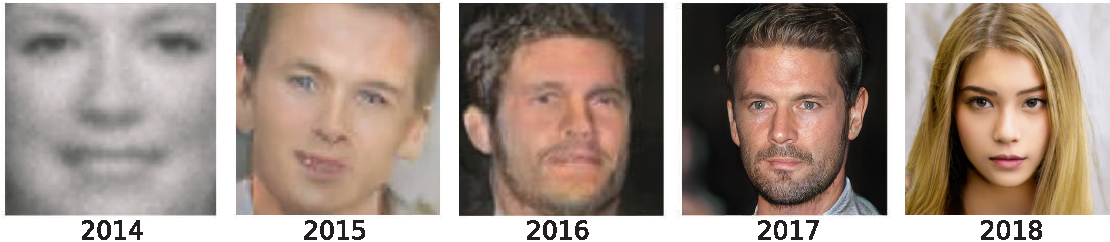
\includegraphics[width=\textwidth]{generative-evolution.pdf}
	\caption{Increasingly realistic qualities of the generated faces using generative adversarial networks as shown in \protect\cite{brundage2018malicious}; images are taken from \protect\cite{goodfellow2014gan}, \protect\cite{radford2015dcgan}, \protect\cite{liu2016cogan}, \protect\cite{karras2017pggan}, and \protect\cite{karras2019stylegan}.} 
	\label{fig:generative-evolution}
\end{figure}


Inherently, unsupervised learning is less well-defined than supervised learning, and this is the reason why unsupervised learning is sometimes synonymous with clustering, because finding clusters is usually as much an unsupervised learning system can do.
However, the recent success of deep learning introduced a new breed of generative models, enabling the end-to-end generation of complex data such as photos and audio signals.
\emph{Generative adversarial networks} (GAN) \cite{goodfellow2014gan} are the most notable among them, and their performance in generating realistic images has been improving at an extraordinary pace, as shown in Figure \ref{fig:generative-evolution}.
Combined with the various techniques for manipulating the semantic information in GANs as will be introduced in Section \ref{ch:deeplearning}.\ref{sec:gan}, this hints at completely new kinds of generative methodologies for audio processing.


In this context, this thesis aims to design and develop improved methods for automatic music transcription powered by deep generative models.
The idea specifically hypothesizes that by training a generative model, it is possible to learn disentangled representations, from which the information necessary for transcription can be easily extracted, as depicted in Figure \ref{fig:autoencoder}.
By doing so, the ultimate objective is to build an end-to-end differentiable model that connects the piano roll representation to audio signals, in order to perform automatic music transcription --- obtaining the most likely piano roll representation for given a audio waveform.


\subsection{On the Broader Context of Machine Listening in AI Research}

Using generated audio data and generative models is partly motivated by the fact that synthesized music is more prevalent and perceptually more familiar to people than synthesized texts or pictures.
Many commercial music tracks are often produced entirely using software instruments, except for the vocal parts.
This suggests that synthesized and generated audio may more accurately model the distribution of the real audio data to be transcribed.
This generative approach also aligns well with how actual musicians transcribe music, where they match given audio with their knowledge of how the instruments sound when played in a certain combination of rhythms and melodies.
Therefore it is reasonable to claim that machines should also be able to perform in a similar way, provided that a proper representation of knowledge about the music and instruments is available.

The task of automatic music transcription shares many common values with other machine learning tasks, such as image segmentation, machine translation, and speech recognition, in the sense that the core task is to build an intelligent system that can extract and process useful information conveyed in complex signals.
This is an essence of artificial intelligence (AI)
--- a system that perceives its environment and takes actions that maximizes the utility \cite{russell2009ai} --- 
where an intelligent system has to understand the semantics of complex data coming from the environment in order to perform well in its tasks.
To this end, the problem of automatic music transcription is not just an intriguing task in music technology but will also be a key component of the AI-enabled future society, constituting a musical component of the artificial general intelligence (AGI), in the form of advanced machine musicianship \cite{rowe2003musicianship}.


\subsection{Organization of The Thesis}


This thesis examines the possibility of using deep generative models to learn relevant musical concepts and inform a music transcription model to incorporate them.
There exists a rich history of research aiming at the understanding of musical sounds and automatic music transcription; to validate this claim as a feasible research direction and place this thesis in the context of this continuum of research, Chapter \ref{ch:mir} provides a review of the standard methods and the current state of the art in automatic music transcription research.
Deep learning techniques are employed as a building block throughout this thesis, and a general introduction to deep learning and deep generative models is provided in Chapter \ref{ch:deeplearning}, with a focus on generative adversarial networks.

In Chapter \ref{ch:monophonic}, we first consider a subproblem of music transcription, i.e. monophonic pitch estimation, and learn that convolutional neural networks predicting two-dimensional time-frequency representations can constitute an effective strategy, which we build and extend in the subsequent chapters.
Chapter \ref{ch:synthesis} examines the applications of deep generative models in music analysis and synthesis tasks, by introducing a WaveNet-based music synthesis model that learns a multi-dimensional timbre representation.
In Chapter \ref{ch:adversarial}, generative adversarial networks are used to apply a music language model that can help improve a piano transcription model.
In Chapter \ref{ch:timbre}, we combine the analysis and synthesis methods developed in the preceding chapters and present a multi-instrument polyphonic music transcription system.
Finally, concluding remarks are provided in Chapter \ref{ch:conclusions}.



%!TEX root = ../dissertation.tex
% this file is called up by thesis.tex
% content in this file will be fed into the main document

%: ----------------------- introduction file header -----------------------
% the code below specifies where the figures are stored
\graphicspath{{2-review/figures/}}

\chapter{Review of Related Literature}
\label{ch:review}


\section{Deep Learning in a Nutshell}\label{sec:deeplearning}

Since recently, a family of machine learning research under the buzzword "deep learning" has incurred groundbreaking changes to the world of artificial intelligence, making the long-waited dream of the strong artificial intelligence look not so distant in the future.
The impact of deep learning was so dramatic that many successful applications of deep learning like DeepMind's AlphaGo beating the human Go champion and Google's neural machine translation have became familiar to laypeople.
The core idea of using artificial neural network to process complex information traces back to the very early days of computing \cite{kleene1951representation}, but it has long been considered less effective than alternative methods, such as support vector machines or probabilistic graphical models.
Around 2010, it turned out that neural networks can substantially outperform those other approaches and have much more flexibility for the further improvements, and the lower performance of neural network was simply due to the insufficient data, the lack of computational power, and some tricks that have not been employed before.
This finding has opened the era of deep learning, a term coined after the fact that neural networks often employ multiple layers of learned feature transformations, and is continuing to innovate virtually all fields of science and engineering, including, of course, music technology.

Because it is expected that the methodologies and techniques of deep learning will play a crucial role in the thesis, this section briefly covers the essential concepts and terminologies of deep learning. Starting from the basic architectures and techniques, more emphasis will be given on manifold learning and deep generative models, as these are the key concepts and techniques that enables the generation of natural-sounding music.

\subsection{Neural Network Architectures}

The key idea of artificial neural network is basically to find an appropriate matrix $W$ to model the relationship between variables $\mathbf{x}$ and $\mathbf{y}$ so that
\begin{equation}\label{eqn:perceptron}
	\mathbf{y} = \sigma(W \mathbf{x})
\end{equation}
is a good approximation, where $\sigma$ is a nonlinear function like sigmoid or hyperbolic tangent. This model in Equation \ref{eqn:perceptron} is also known as a perceptron \cite{rosenblatt1957perceptron}, one of the first artificial neural network to be produced.
This computation --- a matrix multiplication followed by a nonlinear activation --- can be applied multiple times, like
\begin{equation}\label{eqn:mlp}
	\mathbf{y} = \sigma(W_3\sigma(W_2 \sigma(W_1 \mathbf{x})))
\end{equation}
which gives the model more expressive power.
This model in Equation \ref{eqn:mlp} is called a multilayer perceptron (MLP) in a sense that it is a concatenation of perceptrons, and the fact that it contains multiple layer is why these neural networks are called "deep".

A multilayer perceptron is a special case of feedforward neural network, which refers to any computational graph that does not contain a cycle. A popular model under this category is convolutional neural networks (CNN), which uses a convolution (a cross-correlation, to be precise) with a fixed-size kernel instead of the fully connected layers performing matrix multiplications.
This results in a fewer number of parameters to learn in each layer, allowing deeper models for the same total number of parameters.
LeNet \cite{lecun1995lenet} for digit classification is what pioneered the technique of using convolutional layers in neural networks, and it is an essential building block of the majority of deep learning methods, including the models that surpassed the human-level accuracy in the ImageNet Large Scale Visual Recognition Challenge (ILSVRC) \cite{krizhevsky2012imagenet, simonyan2014vgg, szegedy2015googlenet, he2016resnet}.
Fully convolutional networks, which omit the fully connected layers that are typically placed at the last stages of neural networks, do not require a fixed input and output size and are known to perform well for image segmentation \cite{long2015fully}.
Because deep convolutional layers are known to be capable of extracting complex semantic information from images, many artistic applications have been developed, such as the transfer of artistic style from one image to another \cite{gatys2015style}, and a captivating visualization known as Deep Dream \cite{mahendran2016deepdream}.

A network with a cyclic connection is called a recurrent neural network, and has been successfully applied to modeling sequence data.
Because it is hard for a recurrent neural network to propagate long-range dependencies through a chain of recurrent connections, a specific recurrent unit called long short-term memory (LSTM) \cite{hochreiter1997lstm} and gated recurrent unit (GRU) \cite{cho2014seq2seq} are devised to resolve the problem and are considered essential for recurrent neural network.
A specific formulation of recurrent neural network called the sequence-to-sequence model \cite{cho2014seq2seq,sutskever2014seq2seq} is well known to be very effective for machine translation, and is deployed in production in Google's translation services \cite{wu2016google}.

Reinforcement learning \cite{sutton1998reinforcement} is a formulation of machine learning where a software agent takes actions in an environment to maximize the reward given according to the actions.
This formulation is inspired by behaviorist psychology and is well-suited for environments that require explorations by the agent, such as robotics and games.
Deep Q-Network (DQN) \cite{mnih2015dqn} is a neural network model designed for reinforcement learning, which has been successfully applied to automatically playing Atari games \cite{mnih2013atari} and the agent playing the game of Go that surpassed the human level \cite{silver2016alphago}.

\subsection{Techniques for Better Performance and Faster Optimization}

Training a neural network involves optimization of its parameters, e.g. $W$ in Equation \ref{eqn:perceptron} and \ref{eqn:mlp}, which typically requires the gradient of the loss function, i.e. the partial derivatives with respect to all of the model's parameters.
It is feasible to manually derive the gradient for shallow models, but for deep neural networks it is often too complex and error-prone to calculate the derivative by hand.
For this reason, a method called backpropagation \cite{werbos1982backpropagation, williams1986backpropagation} was introduced based on the ideas of automatic differentiation \cite{linnainmaa1970ad} and revived neural network research that had been largely abandoned since 1970.
The popularization of backpropagation in the 1980s partly contributed to the ending of the first AI winter, leading to the first commercially successful application of neural network in optical digit recognition and speech recognition.
Backpropagation is still an elemental part of deep learning, and many deep learning frameworks are capable of automatically calculating gradients using backpropagation when a compute graph is given.
This enables the developer to write only the forward calculation and run the backpropagation automatically, greatly improving the productivity.

Once a gradient is known the standard way of optimizing a neural network is to use a variant of stochastic gradient descent, where the direction of the gradient descent is determined only based on a mini-batch of training data.
Although using only a subset of training data will make the gradient unstable, practically it is known to converge faster with the stochastic version.
Adding momentum in the gradient descent optimizer has shown to be effective for finding the convergence even faster, and many schemes for applying the momentum have been introduced, such as Adagrad \cite{duchi2011adagrad}, RMSprop \cite{tieleman2012rmsprop}, Adadelta \cite{zeiler2012adadelta}, Adam \cite{kingma2014adam}, and Eve \cite{koushik2016eve}.

Historically, sigmoid and hyperbolic tangent function have been popular choices for the nonlinearity, but it is surprisingly shown \cite{nair2010relu} that rectified linear units (ReLU),
\begin{equation}
	f(x) = \max \{ x, 0 \},
\end{equation}
generally improves the accuracy of deep learning models.
It is also known that neural networks with ReLU activations converge faster, and more robust to vanishing gradient problem.
A number of ReLU variants, including leaky ReLU \cite{xu2015leakyrelu}, parametric ReLU (PReLU) \cite{he2015prelu}, SReLU \cite{jin2015srelu}, have been devised and successfully applied to various tasks.

As with any other machine learning methods, overfitting is a problem to overcome for deep learning models as well.
While directly adding a L1 or L2 regularization term of weights is possible, a few cleverer tricks for preventing overfitting have been devised and widely employed, and they are treated as regularization methods in a wider sense.
Dropout \cite{srivastava2014dropout} is a simple yet powerful regularization method that turns off a random subset of activations during the training process.
Because the network has to learn how to make accurate predictions using only a random subset of its components, the training becomes more robust and less susceptible to overfitting.
Batch normalization \cite{ioffe2015batchnorm} is a method to reduce the covariance shift by performing normalization for each training mini-batch, and is also known to improve the generalizability of the trained model.
Despite being relatively new, dropout and batch normalization are drop-in methods that can be added to most deep architecture with almost no changes of code and yet significantly improve the performance, and are thus included almost by default in the majority of newer deep models.

Additionally, because typical neural networks contain thousands to millions of parameters to train, a proper initialization of the weights prior to training is important.
In early days of deep learning, unsupervised pre-training of weights \cite{bengio2007greedy,erhan2010pretraining} was considered necessary, but recently it is shown that a simple random initialization of weights is sufficient with the current computational power of the hardware.
A widely practiced way of initializing the weights without unsupervised pre-training is to sample from a Gaussian or uniform distribution according to the number of input and output nodes \cite{glorot2010initialization,he2015prelu}.

\subsection{Manifold Learning and Deep Generative Models}

A natural formulation of neural network for unlabeled data is to build an encoder that transforms the input data into a smaller dimension, followed by a decoder that maps it back to the original data.
This architecture is called an autoencoder \cite{bengio2009deeplearning}, and is capable of learning a nonlinear mapping for dimensionality reduction.
Variants of the autoencoder architecture include sparse autoencoder \cite{ng2011sparse} that produces a sparse representation of the input data, denoising autoencoder \cite{vincent2008denoising} that is capable of reducing noise or recover redacted portion of an image, and contractive autoencoder \cite{rifai2011contractive} that adds a regularization term to make the model robust to slight variations of input values.

The idea of stacking an encoder and a decoder together is applied to many generative models.
In variational autoencoder (VAE) \cite{kingma2013vae}, the encoder predicts the posterior distribution of data that is restricted to be multivariate Gaussian, and the decoder reconstructs the input data from the samples of the Gaussian distribution.
VAE can be used to generate data samples from Gaussian noise, and thus classified as a generative model.
However, there are many limitations of VAE that led to blurry reconstructed images, that may come from the inexactness of the Gaussian assumption and the variational lower bound used by the model \cite{doersch2016tutorial}.

Another family of deep generative models that have become extremely popular since the last year is generative adversarial network (GAN) \cite{goodfellow2014gan}.
Unlike other deep neural networks models that use optimization to find the weights minimizing the loss function, GANs try to find a Nash equilibrium between its two components, the generator and discriminator.
Given the training data $\mathbf{x}\sim p_{\mathrm{data}}$ and the latent distribution $\mathbf{z} \sim p_z$ which typically is a multivariate Gaussian distribution, GAN performs the following minimax game:
\begin{equation}\label{eqn:gan}
	\min_{G} \max_{D} \Big[ \mathbb{E}_{\mathbf{x} \sim p_{\mathrm{data}}} {\log D(\mathbf{x})} + \mathbb{E}_{\mathbf{z} \sim p_z} \log \left ( 1 - D(G(\mathbf{z})) \right ) \Big],
\end{equation}
where the generator learns to transform a noise vector $\mathbf{z}$ into a data point that can fool the discriminator as if it is a real data sample, while the discriminator tries to correctly distinguish the output of generator $G(\mathbf{z})$ from the real data $\mathbf{x}$.
Some variations of the minimax game in Equation \ref{eqn:gan} are introduced in \cite{goodfellow2016gan}.

Since the introduction of GAN, a lot of its variants and applications have been introduced at an astounding pace.
As the original GAN architecture was not capable of learning from high-resolution images, LAPGAN \cite{denton2015lapgan} uses a Laplacian pyramid of images for generating high-resolution images, and Deep Convolutional GAN (DCGAN) \cite{radford2015dcgan} follows a list of best practices that are considered to be helpful in training GAN for large images.
A number of practical and theoretical insights were introduced in order to help make GAN training more stable, where researches suggested a list of improved techniques \cite{salimans2016improved}, included various regularization terms in the minimax game \cite{che2016mrgan}, and used Wasserstein distance instead of the usual Kullback-Leibler distance GAN \cite{arjovsky2017wasserstein,berthelot2017began}.
There also have been a number of variants to make the latent representation to convey an interpretable semantic of the data, e.g. Conditional GAN \cite{mirza2014conditional}, Auxiliary Classifier GAN \cite{odena2016acgan}, Adversarially Learned Inference \cite{dumoulin2016ali}, and InfoGAN \cite{chen2016infogan}.
GANs are also known to be successful in transferring artistic style \cite{zhu2017unpaired} and other cross-domain relationships \cite{kim2017discogan} as well as speech enhancement \cite{pascual2017segan} which is notable because it works directly on the time-domain audio signal using 1-D convolutions.

The amazing performance of GAN is not yet grounded by a perfect theoretical interpretation, but it is conjectured that GAN performs well because it can precisely model the lower-dimensional manifold that contains the data, unlike VAE which assumes a Gaussian posterior and includes a variational lower bound that results in blurry generated images.
For example, the distribution of the MNIST digit images \cite{lecun1998mnist} is much lower dimensional than the actual 784-dimensional distribution of the bitmap images, and even a 2-D t-SNE embedding \cite{maaten2008tsne} can map the entire 60,000 images to a 2-D space while almost perfectly separating the digit labels.
This manifold assumption should also hold for music signals, and deep generative models should be able to find such manifold which enables an easier extraction of semantic information for music transcription.
An early proof of this is in Figure \ref{fig:tsne}, which shows that a convolutional neural network trained to classify the instruments of Vienna Symphonic Library can learn a manifold that separates the sounds according to the family of instruments.

Extending this result, the core idea of this thesis is to build a deep generative model that learns a manifold that conveys richer information about the musical sound, including not only the family of instruments but also pitch, rhythm, and dynamics which are the elements of music transcription.

\begin{figure}
	\centering
	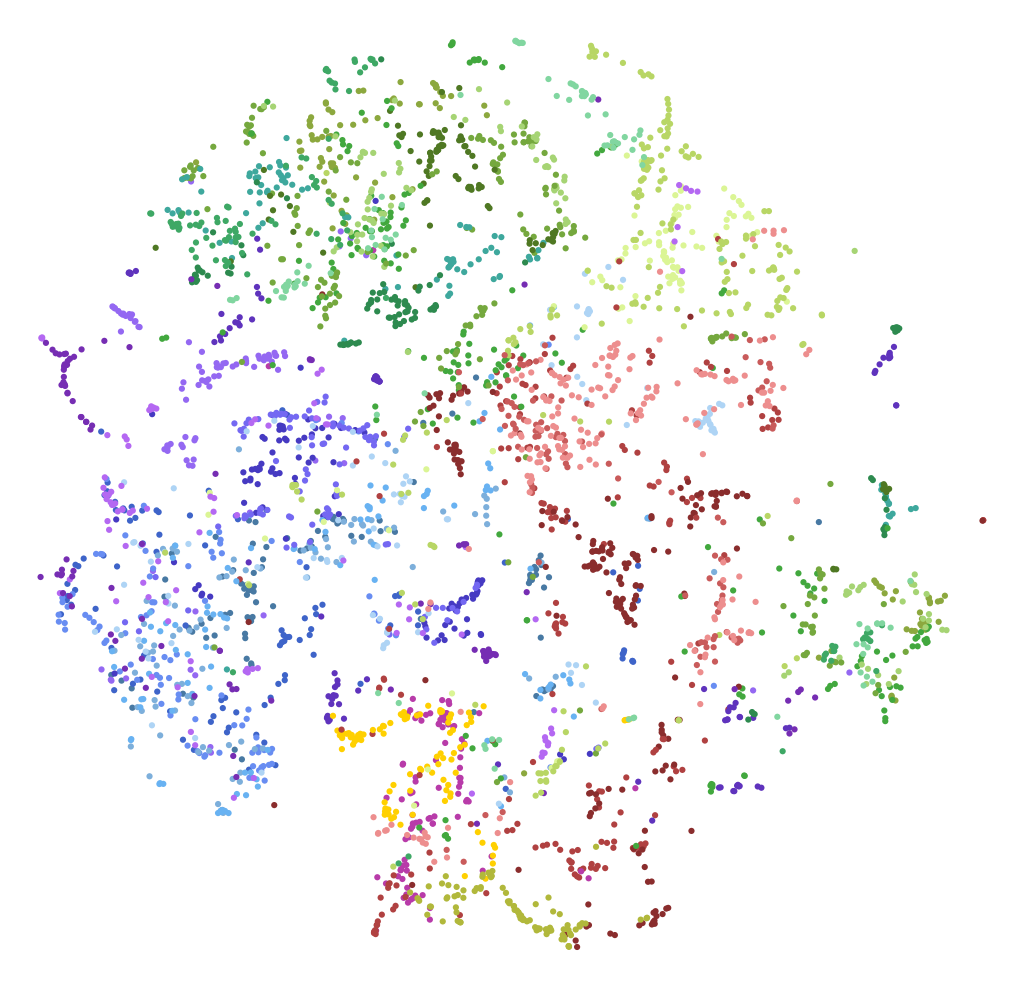
\includegraphics[width=0.55\textwidth]{instruments-tsne.png}
	\caption{A 2-D t-SNE embedding of sounds from Vienna Symhonic Library shows that a convolutional neural network can learn a manifold that separates the sounds of woodwinds (blue colors), strings (red colors), and brass (green colors) instruments.}\label{fig:tsne}
\end{figure}






\section{Music Information Retrieval Methods for Transcription} \label{sec:review}

Being able to accurately identify all musical events from audio and transcribe them into musical notations is an essential skill for musicians as well as a paramount goal of music machine learning research.
Enabling an automatic conversion from musical audio to symbolic notations, and vice versa through music synthesis, opens up many new possibilities.
The most straightforward application of automatic music transcription would be a software tool that transcribes audio recording and produces a musical score, which can aid musicians in various situations.
Automatic music transcription can help build a melody database to be used for music retrieval systems, such as query by humming \cite{molina2014humming}, where it is often very hard to obtain annotated data even when the audio files are abundantly available.
Similarly, by building a database containing symbolic information of music, music recommender systems can leverage the database to infer how much individual users would prefer the music, based on melodic, harmonic, and instrumental information present in the transcription.

As stated, due to the complexity and difficulty of creating an all-encompassing end-to-end music transcription system, many existing approaches focus on a specific subtask of the problem \cite{casey2008mir}, e.g. extracting onsets and beats, recognizing timbre and instruments, tracking monophonic and polyphonic pitches, or separating audio sources from a mixture.
Each of these subtasks poses interesting goals and applications even without the lofty goal of the full music transcription, and they are often classified under the umbrella term of music information retrieval (MIR).
Although this term has existed since 1960s \cite{kassler1966mir}, it was only after the late 1990s when active research on this area has spun off from computer music and computational musicology literature.
During the last two decades, numerous sophisticated and novel approaches for each of these subproblems have been introduced, that have continuously improved the performance in terms of the accuracy in predicting the correct annotations.
This section will first introduce the standard pipeline of music information retrieval, followed by a few state-of-the-art techniques for music transcription.

\subsection{The Standard Pipeline}

Audio data is huge in volume --- a typical audio track contains 44,100 real-numbered samples per second, and sometimes even more.
Therefore, computational methods for extracting musical information from audio usually contains a pipeline of feature extraction stages to reduce the volume and increase the interpretability of input data, as shown in Figure \ref{fig:pipeline}.
The pipeline shares many techniques that have been widely used in speech processing, but also many feature extraction stages are created for music-specific purposes.

\begin{figure}[t]
	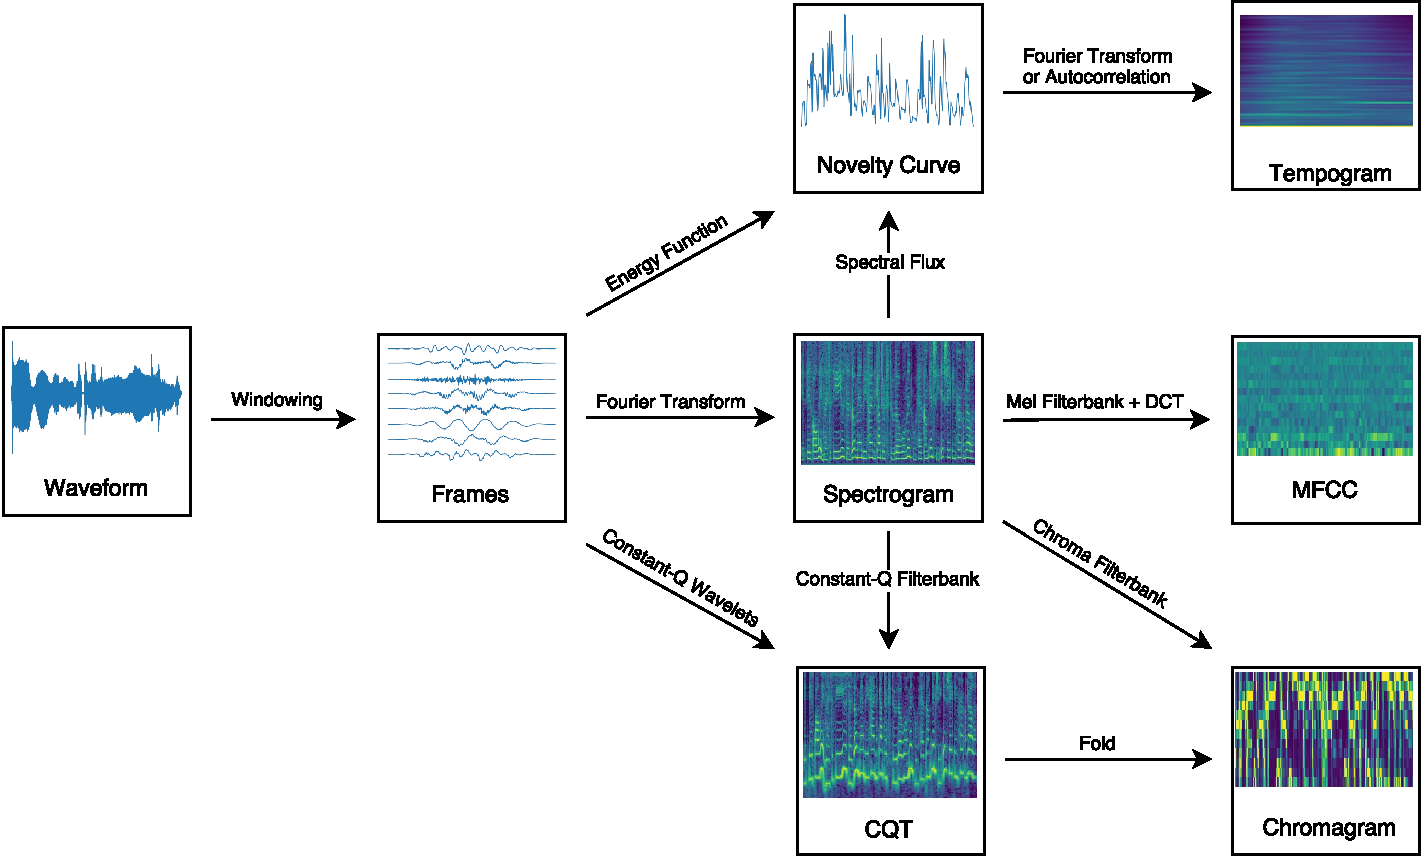
\includegraphics[width=\textwidth]{pipeline.pdf}
	\caption{\small The standard pipeline for music feature extraction. An appropriate set of feature extraction methods needs to be heuristically selected depending on the task.}\label{fig:pipeline}
\end{figure}

While there are many MIR tasks that operate on the track-level, such as music recommendation, tagging, and genre classification, most subtasks of music transcription involve the prediction of labels that are dependent on time, operating either in the sample-level or frame-level.
Frames are created by taking a series of overlapping short-time audio segments, where the length of a segment is typically 10-50 milliseconds, and optionally multiplying them by a windowing function.
Taking discrete Fourier transforms on the frames produces a short-time Fourier transform (STFT), and the magnitude of an STFT gives a spectrogram.
Spectrograms give very rich information about the audio; for example, the contour of melodies and dynamics of music are usually identifiable from the image.
However, the dimensionality of a spectrogram is still quite high, making it computationally prohibitive to run many algorithms directly on an STFT or a spectrogram.
This necessitated further transformations by the means of filterbanks, producing Mel-Frequency Cepstral Coefficients (MFCC) via the Mel filterbank, or chroma features by applying 12 filters specific to each scale degree.
Constant-Q transform (CQT) \cite{schorkhuber2010cqt} alleviates a drawback of STFT in which the linear spacing of frequency bins does not align with human auditory perception, by placing the center frequencies of filters to have a constant Q factor, which is the ratio between the center frequency and the 3 dB bandwidth of a filter.
By configuring CQT to produce 12 filters per octave, it is possible to obtain the coefficients corresponding to each musical tone, and to fold the representation to produce a chroma feature.
To extract the beat and tempo information, heuristic functions like the first-order difference of the time-domain log energy function or the spectral flux that measures the total energy increase over the frequency bins, to formulate a novelty curve, which measures energy bursts typically present in the onsets of notes.
The onset information can then be further processed to obtain tempo information via tempograms.


%Although a few recent techniques were successfully applied on the raw audio data without a predefined feature transformation,

While the pipeline shown in Figure \ref{fig:pipeline} is considered a de-facto standard for any audio processing systems, recent deep learning approaches have successfully eliminated some or all feature transformation stages by training model to learn the feature from the spectrogram or audio waveforms.
In theory, any feature extraction stage induces a loss of information, and it suggests that the best-performing model would benefit most from the raw audio data.

\subsection{Techniques for Multiple Fundamental Frequency Estimation}

Among the aforementioned subtasks of automatic music transcription, estimating the pitch from polyphonic recording poses the most difficult challenges, as apparent from the recent stream of results from MIREX challenges \cite{downie2014mirex}.
The task is commonly referred to as multiple fundamental frequency estimation (Multi-F0 estimation, or MFFE), and in some sense supersedes the onset and beat detection problems as well as chord and melody tracking problems,
since the frequency tracking has to indicate the onset and offset of every sound, and tracking chords and melodies becomes much easier when the correct annotations for all pitch contours are available.

Many early methods for MFFE \cite{klapuri2003multiple,emiya2010multipitch} focused on extracting features like harmonicity and spectral smoothness from the audio spectrogram and devising a good heuristic for frequency estimation.
More recent models employ data-driven approaches, using dynamic Bayesian networks \cite{raczynski2013dynamic} or recurrent neural networks \cite{sigtia2016endtoend}, and achieved better performance.

The idea of using generative models to predict multiple fundamental frequencies is not new \cite{dubois2005harmonic,cemgil2006generative}, but they relied on manually designed generative models for sound generation, which might have led to poor generalizability.
Using deep generative models is expected to help overcoming this limitation, since deep learning methods is known to be excellent in learning embeddings and manifolds that are generalizable to different tasks and domains.




%!TEX root = ../dissertation.tex

\graphicspath{{9/figures/}}
\chapter{Conclusion}
\label{chp:conclusion}

\section{Findings}
Carrot cake croissant tart bonbon candy biscuit donut liquorice muffin. 
Jelly beans gummies cheesecake cotton candy bonbon chocolate cake croissant gingerbread macaroon. 
Tiramisu liquorice brownie sesame snaps dragee sugar plum tiramisu jelly-o. 
Pastry bonbon pastry cheesecake applicake powder candy tart. 
Marzipan dessert ice cream brownie wafer cookie marshmallow. 
Carrot cake pudding brownie carrot cake dessert icing brownie chocolate.


\section{Implications}

Sugar plum caramels wafer cotton candy powder cotton candy. 
Caramels lemon drops. 
Bonbon jelly-o pudding macaroon. 
Ice cream applicake tart gummies brownie bonbon jelly beans. 
Gingerbread toffee lollipop tart ice cream brownie.
Chocolate bar gingerbread chupa chups. 


%!TEX root = ../dissertation.tex

\graphicspath{{9/figures/}}
\chapter{Conclusion}
\label{chp:conclusion}

\section{Findings}
Carrot cake croissant tart bonbon candy biscuit donut liquorice muffin. 
Jelly beans gummies cheesecake cotton candy bonbon chocolate cake croissant gingerbread macaroon. 
Tiramisu liquorice brownie sesame snaps dragee sugar plum tiramisu jelly-o. 
Pastry bonbon pastry cheesecake applicake powder candy tart. 
Marzipan dessert ice cream brownie wafer cookie marshmallow. 
Carrot cake pudding brownie carrot cake dessert icing brownie chocolate.


\section{Implications}

Sugar plum caramels wafer cotton candy powder cotton candy. 
Caramels lemon drops. 
Bonbon jelly-o pudding macaroon. 
Ice cream applicake tart gummies brownie bonbon jelly beans. 
Gingerbread toffee lollipop tart ice cream brownie.
Chocolate bar gingerbread chupa chups. 



% -------------------------------------------------------------- 
%:                  BACK MATTER: appendices, refs,..
% --------------------------------------------------------------

% the back matter: appendix and references close the thesis


%: ----------------------- bibliography ------------------------

%\clearpage
\onehalfspacing
\bibliographystyle{apacite}

\renewcommand{\bibname}{Bibliography} % changes the header; default: Bibliography

\bibliography{backmatter/library} % adjust this to fit your BibTex file



%: ------ appendices----------------------------------------
\appendixbegin
\appendix

\chapter{Brownie tootsie roll lollipop cookie}
\label{adx:a}

\doublespacing

Oat cake pudding sweet lemon drops gummies cookie. 
Dragee lollipop ice cream apple pie sweet roll brownie. 
Lollipop marshmallow jelly beans marzipan sugar plum chupa chups caramels toffee. 
Croissant icing chocolate cake oat cake muffin powder tart. 
Croissant wafer dessert pudding cupcake croissant. 
Cheesecake wafer sugar plum danish. 
Liquorice powder sesame snaps.


%: --------------------------- index ---------------------------

%\clearpage
% \begin{footnotesize}
% \cleardoublepage % ensure the right page
% \phantomsection % sets an anchor
% \printindex
% \end{footnotesize}



\end{document}
